\documentclass[conference]{IEEEtran}
\IEEEoverridecommandlockouts
% The preceding line is only needed to identify funding in the first footnote. If that is unneeded, please comment it out.
\usepackage{cite}
\usepackage{amsmath,amssymb,amsfonts}
\usepackage{algorithmic}
\usepackage[utf8]{inputenc}
\usepackage{graphicx}
\usepackage{textcomp}
\usepackage{xcolor}
\usepackage{makecell}
\def\BibTeX{{\rm B\kern-.05em{\sc i\kern-.025em b}\kern-.08em
    T\kern-.1667em\lower.7ex\hbox{E}\kern-.125emX}}
\begin{document}

\title{Network Term Project Part 2 \\
{\textsuperscript{Group 29}}
\thanks{}
}

\author{\IEEEauthorblockN{İbrahim Atacan KERPİÇ}
\IEEEauthorblockA{2099174}
\and
\IEEEauthorblockN{Yusuf TOPÇUOĞLU}
\IEEEauthorblockA{2099398}
}

\maketitle

\section{Introduction}
In this assignment, we have designed and implemented a network which consists of a source node, a broker (B), routers and a destination node. We are sending a large file (exactly 5.000.000 bytes) from source to destination. The Source sends packets to Broker via TCP. Between Broker and Destination, our RDT protocol is working on top of UDP. 

\section{Purpose of the Project}
The purpose of this project is to learn reliable data transfer protocol basics like timeout, retransmission, and packet order. We have learned to implement reliable data transfer protocol in python and we reinforce our TCP, UDP socket programming knowledge along with the GENI platform, SSH, SCP, and TMP protocols.  

\section{Design Process}

In our project, we have three nodes that will run scripts and two routers that will route the packets to the next hop.

We have designed our routers so that they forward the packets directly to the next hop as it is stated in the homework text. Forwarding tables and configuration commands are in the readme file.

Since the communication between the Source and Broker is TCP, we are sure that packets that we send from the Source to the Broker will receive correctly and in order. The Source node first sends the whole file to the Broker. While Broker gets the packets from the Source, it does not start to send, but first stores the whole packets. Then, the broker can guarantee to send the packets to the destination correctly and in order by using our RDT protocol.

We design our protocol to be a UDP-based "Reliable Data Transfer" (RDT) protocol that supports pipelining and multi-homing. To support pipelining functionality, we preferred  "go back-n" protocol since we think it meets the homework's requirements about pipelining. We have explained how the "go back-n" protocol provides pipelining functionality under the "Algorithms and Strategies" section.

Similarly, to make our project support multi-homing, we design our Broker and Destination working algorithm to use both r1 and r2. Therefore, we split the traffic between r1 and r2 equally. This approach also explained under the "Algorithms and Strategies" section in more detail.

We have used the timeout mechanism to detect lost packets and retransmit those packets as it is in the "go back-time", and sequence numbers to ensure the correct order of packets while designing the RDT protocol functionality of our project. 

\section{Implementation Process}
We choose python3 as a programming language for the implementation process.

We continue from our previous part 1 implementation. The first minor change was to read and send a file over the network in the source implementation and write the result to an output file in the destination side. The headstones of the implementation of our protocol for each script is explained in subsections.

\subsection{Source (source.py)}

\begin{table}[h]
\renewcommand{\arraystretch}{1.3}
\caption{Global and/or Important variables of Source}
\label{tab:example}
\centering
\begin{tabular}{c|c}
    \hline
    Name &  Description\\
    \hline
    \hline

    file$\_$object   &   The file object that will be sended to the destination.\\
    \hline

    payload$\_$size    &   The size of packets that are sended to the broker.\\
    \hline
\end{tabular}
\end{table}

We opened the file that will be sent to the destination. Then we set the Broker’s host address and the port. We created a TCP socket and an address object with the host address and port number of Broker. Then, connection is established between source and broker with tcp socket. After the connection, in a while loop, we read and send the file with the payload size until the whole file is sent in.

\subsection{Broker (broker.py)}

\begin{table}[h]
\renewcommand{\arraystretch}{1.3}
\caption{Global and/or Important variables of Broker}
\label{tab:example}
\centering
\begin{tabular}{c|c}
    \hline
    Name &  Description\\
    \hline
    \hline

    nextseqnum   & \makecell{Sequence number of the next packet \\ that will be sent.} \\
    \hline

    base    &   \makecell{The oldest sent but not ACKed packet.}\\
    \hline
    
    wnd$\_$size    &  \makecell{The number indicating how many not ACKed \\packet can be send consecutively.} \\
    \hline
    
    snd$\_$pkt    &   \makecell{The array that contains all of the \\ packets that will be sent.} \\
    \hline
    
    sample$\_$rtt    &   \makecell{The sample round trip time value.}\\
    \hline
    
    estimated$\_$rtt  &  \makecell{The estimated round trip time value}\\
    \hline
    
	dev$\_$rtt    &   \makecell{The deviation value of round trip time.}\\
    \hline    
    
    total$\_$packet$\_$count  &  \makecell{Total number of packets that will be sent.} \\
    \hline
    
    sent$\_$time    &   \makecell{Start time of RTT.} \\
    \hline
    
    is$\_$acked    &   \makecell{Flag indicating that this measurement  \\ of RTT finished or not.  }\\
    \hline
    
    received$\_$time    &   \makecell{End time of RTT.}\\
    \hline
    
    payload$\_$size    &   \makecell{The size of packets payload.}\\
    \hline
    
    timeout$\_$interval    &   \makecell{The interval of timeout.}\\
    \hline
    
    lock    &  \makecell{The lock object that provides concurrency.}\\
    \hline
    
    timer    &  \makecell{"threading.Timer" object that initiates timeout \\ function after "timeout$\_$interval" amount of time\\ has passed after it started}\\
    \hline
    
    
\end{tabular}
\end{table}

When Brokers receives TCP request from the Source, the "handle" method of "ThreadingTCPRequestHandler" class starts to execute. First, it gets the whole file in payload size chunks, prepares the packets that will be sent and stores them into snd$\_$pkt array. This made the retransmission process easy.

\pagebreak

When packets are ready, we start to send them to the Destination over r1 and r2 in a while loop. Here the problem was that broker sends the packets too fast and destination could not handle incoming packets in the correct order because too many threads are working at the same time. As a result, too many timeout and retransmission happened.  We solve this problem by putting a sleep statement in the while loop that sends packets. This made the scenario more realistic and worked more compatible.  Inside the while loop, we implemented "go back-n" protocol.

For every incoming request from the destination,  the "handle" method of "ThreadingUDPRequestHandler" class is executed. When an ack packet received, the "time$\_$out$\_$interval" variable is updated. For the not corrupted incoming ack packets, the receiver side of the "go back-n" protocol is implemented

While implementing the broker.py, we faced with concurrency problems because a new thread handles every incoming packet, meaning more than one thread runs and access to the same variables at the same time. We solved this problem using "threading.Lock" objects. Before accessing the common object, we hold the lock and prevent other threads to access the same variables.

We implement the approach that is stated in the course's textbook under section 3.5.3 while calculating the timeout interval. The approach is the following. The sampleRTT, denoted by sample$\_$rtt in our code, for a segment is the amount of time between when the segment is sent (that is, passed to IP) and when an acknowledgment for the segment is received. Instead of measuring a SampleRTT for every transmitted segment, we take only one sampleRTT at a time. Therefore, we measured time sampleRTT at every round trip time. The estimatedRTT, denoted by an estimatedRTT in our code, is the weighted average of the previous value of estimatedRTT and the new sampleRTT. [RFC 6298] defines the RTT variation, denoted by devRTT in our code, as an estimate of how much SampleRTT typically deviates from EstimatedRTT. Now we can determine the TimeoutIntervaltime, denoted by  time$\_$out$\_$interval in our code. Clearly, the interval should be greater than or equal to EstimatedRTT, or unnecessary retransmissions would be sent. But the timeout interval should not be too much larger than EstimatedRTT; otherwise, when a segment is lost, our protocol would not quickly retransmit the segment, leading to large data transfer delays. It is therefore desirable to set the timeout equal to the EstimatedRTT plus
some margin. The margin should be large when there is a lot of fluctuation in the SampleRTT values; it should be small when there is little fluctuation. The value of DevRTT should thus come into play here. All of these considerations are taken into account in our protocol’s method for determining the retransmission timeout interval:

TimeoutInterval = EstimatedRTT + 4 • DevRTT

An initial TimeoutInterval value of 1 second is recommended [RFC 6298].


\subsection{Destination (destination.py)}


\begin{table}[h]
\renewcommand{\arraystretch}{1.3}
\caption{Global and/or Important variables of Broker}
\label{tab:example}
\centering
\begin{tabular}{c|c}
    \hline
    Name &  Description\\
    \hline
    \hline

    exp$\_$seq$\_$number   & \makecell{ Sequence number of the packet \\ that we expect to receive next.} \\
    \hline

    sndpkt   &   \makecell{The last Ack packet that we send.}\\
    \hline
    
    result   &  \makecell{The variable that we store file before writing the output file.} \\
    \hline
    
    
    lock    &  \makecell{The lock object that provides concurrency.}\\
    \hline
     
\end{tabular}
\end{table}


Destination listens both its own interfaces and opens a new thread for every incoming request. For every incoming request "handle" method of "ThreadingUDPRequestHandler" class is executed. When a packet arrives, we first check if it is corrupted or not. If the packet is not corrupted and has sequence number equal to the expected sequence number, we implemented the "go back-n" protocol of receiver side. However, if the packet is corrupted or not have the sequence number equal to the expected sequence number, we send the "sndpkt" which is the last Ack packet.

Here, we have faced with the concurrency issue as we had in the broker implementation. We solved the problem as we did in the broker, that is, we declared a lock object and acquired the lock before accessing the common elements.

Another problem was to understand when the whole file is received and it is time to write the result to the output file. We have overcome this problem by putting a finish flag to the header, indicating that no any other packet left and the whole packet is finished. We check this flag for incoming packets and understand if the file is received. If the flag is set, we write the result to the output file.

Algorithms and Strategies

\section{Algorithms and Strategies}
In this project, we used "Go Back-N" protocol to support pipelining and RDT mechanisms (checksum, retransmission, ack mechanism, sequence number, timeout mechanism etc)  to provide reliable data transfer.
\subsection{Go Back-N}

Go-Back-N (GBN) protocol is a sliding window protocol. In a Go-Back-N protocol, the sender is allowed to transmit multiple packets (when available) without waiting for an acknowledgment but is constrained to have no more than some maximum allowable number, window size, of unacknowledged packets in the pipeline.

\subsection*{Sender}
• Before sending a new packet, the sender first checks to see if the window is full, that is, whether there are N outstanding, unacknowledged packets. If the window is not full, a packet is created and sent, and variables are appropriately updated. If the window is full, the sender simply tries to send the packet later. 

• Receipt of an ACK. In our GBN protocol, an acknowledgment for a packet with sequence number n will be taken to be a cumulative acknowledgment, indicating that all packets with a sequence number up to and including n have been correctly received at the receiver.

• A timeout event. The protocol’s name, “Go-Back-N,” is derived from the sender’s behavior in the presence of lost or overly delayed packets. A timer will be used to recover from lost data or acknowledgment packets. If a timeout occurs, the sender resends all packets that have been previously sent but that have not yet been acknowledged. Our sender uses only a single timer, which can be thought of as a timer for the oldest transmitted but not yet acknowledged packet. If an ACK is received but there are still additional transmitted but not yet acknowledged packets, the timer is restarted. If there are no outstanding, unacknowledged packets, the timer is stopped.


\subsection*{Receiver}

The receiver’s actions in GBN are also simple. If a packet with sequence number n is received correctly and is in order (that is, the data last saved came from a packet with sequence number n – 1), the receiver sends an ACK for packet n and saves the data portion of the packet. In all other cases, the receiver discards the packet and resends an ACK for the most recently received in-order packet. Note that since packets are saved one at a time, if packet k has been received and saved, then all packets with a sequence number lower than n have also been delivered. Thus, the use of cumulative acknowledgments is a natural choice for GBN.


\subsection{RDT Mechanisms}

We have used known various reliable data transfer mechanisms in our project. We manage lost, corrupted, and out of order packet with those mechanisms.


\subsection*{Lost Packets}

We handle lost packets by using a timeout mechanism. We have a timer in sender-side which is the Broker. We started this timer as it is explained in the GBN protocol and determined the timeout interval as we explained in the Broker's implementation part.

\subsection*{Corrupted Packets}

We handle corrupted packets by using the md5 hashing algorithm. We take the md5 of the whole packet and add this md5 to the end of the packet. Then we control this md5 when we receive the packet on the other side. If they are not equal, we conclude that the packet is corrupted.

\subsection*{Out of Order Packets}
We handle out of order packets by using sequence number strategy. We applied the sequence number strategy as it is explained in the GBN protocol. We count packets as the sequence number in our project.


\section{Packet Structures}



\begin{table}[h]
\renewcommand{\arraystretch}{2}
\caption{Broker to Destination Packet Structure}
\label{tab:example}
\centering
\begin{tabular}{|c|c|c|c|}
    \hline
     \makecell{ Sequence Number \\ 4 Bytes} & \makecell{ FIN Flag \\ 4 Bytes} & Payload & \makecell{ md5 check sum \\ 32 Bytes} \\
    \hline
    
     
\end{tabular}
\end{table}

\begin{table}[h]
\renewcommand{\arraystretch}{1.3}
\caption{Acknowledgment Packet Structure}
\label{tab:example}
\centering
\begin{tabular}{|c|c|}
    \hline
     \makecell{ Sequence Number \\ 4 Bytes} & \makecell{ md5 check sum \\ 32 Bytes}  \\
    \hline
    
     
\end{tabular}
\end{table}



\section{Methodology}


We began our research by looking an example of TCP client and server implementation in python. We then look at to UDP client and server implementation in python. The project includes ''socketserver'' library.

We search the tc and netem commands from the provided homework text.

\section{Motivation}

This project brings us the knowledge of python socket programming and tc \& netem concepts. We experienced to add header to a packet and decompose at the server side. We gain familiarity with the GENI platform and some network concepts like delay, packet lost.

\section{Experiment Results}

\subsection{Netem}
Netem provides Network Emulation functionality for testing protocols by emulating the properties of wide area networks. It emulates variable delay, loss, duplication and re-ordering. Netem is used for the virtuall machines in GENI.

\subsection{NTP}
The Network Time Protocol (NTP) is a networking protocol for clock synchronization between computer systems over packet-switched, variable-latency data networks.

\subsection{Experiments}
First, we add configurations which are mentioned at OdtuClass before each experiment. In order to obtain the file transfer time,  we measured time when the broker receives the first packet from the source. Then, we measured new time when we receive the acknowledgment of the last packet from the destination. The difference gives us the file transfer time.


\subsection*{Experiment 1}

\begin{figure}[h]
\centerline{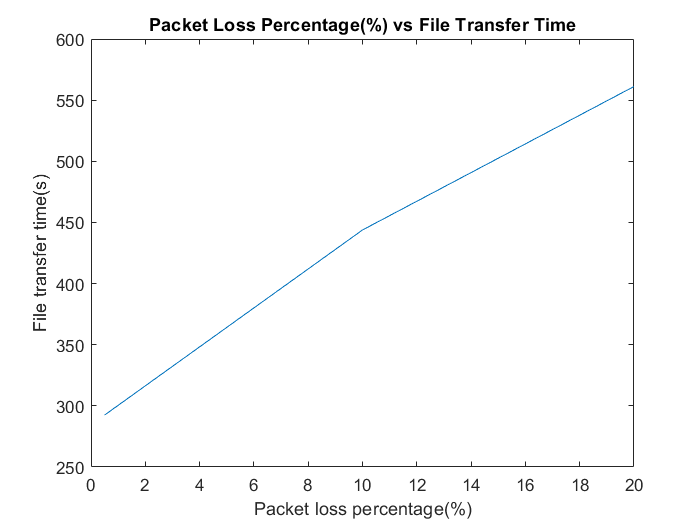
\includegraphics[scale=0.5]{exp1.png}}
\caption{}
\label{fig}
\end{figure}

In the first experiment, we expected that if we increase the percentage of packet loss, file transfer time also will increase because packets that are lost will be retransmitted. The experiment gave parallel results with our expectations. When we increase the percentage of packet loss, some packet are lost as expected, and the timeout happened in broker side. Therefore, lost packets will be retransmitted and file transfer time has increased.

\newpage

\subsection*{Experiment 2}

\begin{figure}[h]
\centerline{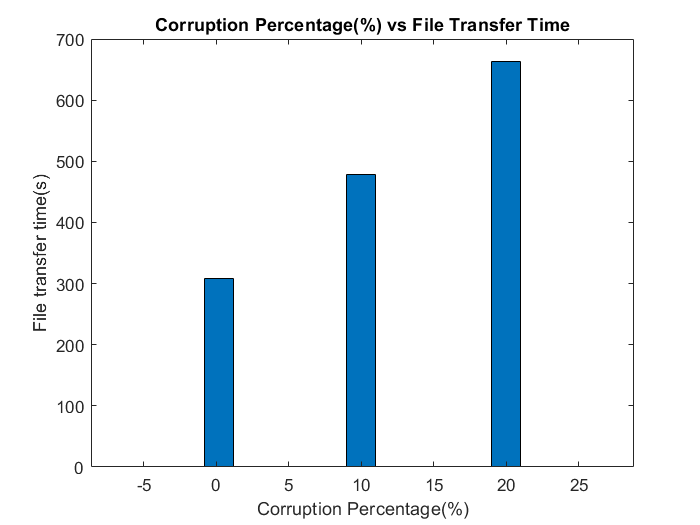
\includegraphics[scale=0.5]{exp2.png}}
\caption{}
\label{fig}
\end{figure}

In the second experiment, we expected that if we increase the percentage of corruption, file transfer time also will increase because packets that are corrupted will be retransmitted. The experiment gave parallel results with our expectations. When we increase the percentage of corruption, our checksum mechanism detected the corrupted packets then the packets were retransmitted.
\subsection*{Experiment 3}

\begin{figure}[h]
\centerline{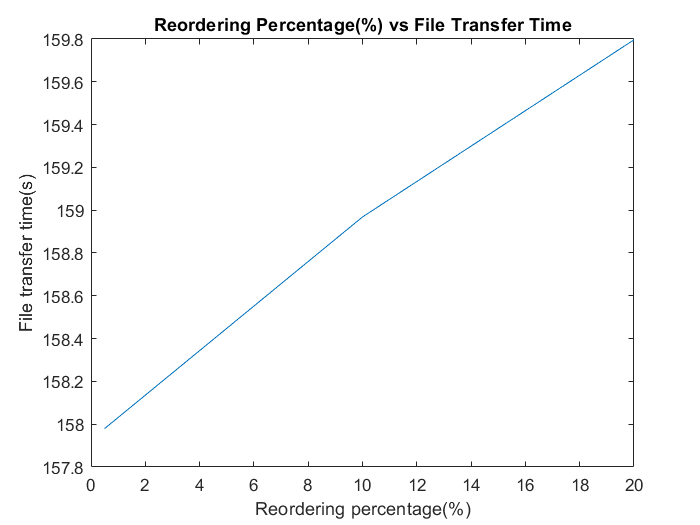
\includegraphics[scale=0.5]{exp3.png}}
\caption{}
\label{fig}
\end{figure}

In the third experiment, we expected that if we increase the reordering, file transfer time also will increase because orders of packets change more frequently and percentage of retransmission will raise. The experiment did not give parallel results with our expectations. When we increase the reordering,  file transfer times are obtained from experiments did not increase as much as we expected. When we read manual page of  tc-netem,  we learned that some of the packets are sent immediately and some of them send with 10 ms delay. This delay doesn't too much affect our execution of scripts because we send packets with 20 ms gaps. 

\section{Workload}

We have performed pair work, we were side by side while developing the project. Hence, the workload was fair.

\end{document}
